
\chapter{Black-box TFNP} \label{chap:bb-tfnp}

\section{Oracles and decision trees}

In the previous chapter we have briefly shown how \TFNP subclasses are defined in terms of basic existence principles that capture white-box total search problems solvable by protocols reducible to Karchmer-Widgerson games. From now on, we will shift our focus to the black-box model.

Black-boxes have been used by complexity theorists since early days, mostly through the concept of \textbf{oracle}, a device capable of instantly solving an instance of a designated problem. In particular, these problems may even be uncomputable, an assumption that allows us to view oracles as a magical devices. Turing machines can be allowed to query such oracles to an additional \textit{oracle tape}. The machine writes a string on such tape, asking the oracle to solve the problem for that input. The output of the oracle is then written on the same tape, which can then be read by the Turing machine. Any query made to the oracle requires $\Theta(1)$ time, meaning that they don't influence the cost of the computation.

\begin{definition}
    An oracle for a problem $A$ is an external device that is capable of instantaneously solving an instance of $A$. An oracle Turing machine is a Turing machine provided with the ability of querying an oracle. We write $M^A$ to describe a Turing machine provided with an oracle for the problem $A$.
\end{definition}

Given a class $\mathcal{C}$ and an oracle for a problem $A$, the \textit{relativized version} of the class $\mathcal{C}$, written $\mathcal{C}^A$ is the set of all problems of $\mathcal{C}$ solvable (or verifiable) with access to the oracle of $A$. For example, $\mathsf{P}^{\mathrm{SAT}}$ is the class of problems solvable in polynomial time by a Turing machine with an oracle for the $\mathrm{SAT}$ problem. More generally, given two classes $\mathcal{C}, \mathcal{B}$, we write $\mathcal{C}^{\mathcal{B}}$ to denote the set of all problems of $\mathcal{C}$ solvable (or verifiable) with access to an oracle for any problem that lies in $\mathcal{B}$. In other words, we have that $\mathcal{C}^{\mathcal{B}} = \bigcup_{A \in \mathcal{B}} \mathcal{C}^{A}$.

Oracles proved to be surprisingly useful for studying the relationship between $\mathsf{P}$ and $\mathsf{NP}$ by considering the relationship between $\mathsf{P}^A$ and $\mathsf{NP}^A$ for an oracle $A$. In a celebrated result \cite{relativization_p_np}, Baker et al. showed that there are two problems $A$ and $B$ such that $\mathsf{P}^A = \mathsf{NP}^A$ and $\mathsf{P}^B \neq \mathsf{NP}^B$. This fact makes commonly used proof techniques useless, meaning that any answer to the $\mathsf{P} \stackrel{?}{=} \mathsf{NP}$ question will require unconventional techniques, thus the hardness of the question.

Oracles provide a simple yet effective way to generalize the concept of reduction through the so called \textit{Turing reductions}: if a Turing machine provided with an oracle for the problem $B$ is capable of resolving a problem $A$ then the problem $A$ can be reduced to solving multiple instances of the problem $B$. When $A$ is Turing reducible to $B$, we write $A \leq_T B$. Clearly, if the oracle machine $M^B$ can solve $A$ then any query to the oracle can be replaced with a call to a subroutine that solves $B$. This conversion is ofter referred to as \textit{de-relativization}. Many-to-one reductions can be seen as a specific case of Turing reductions, where the machine makes exactly one query to the oracle and then returns the the output of such query.

In the particular case of total search problems, it was proven that the reducibility between search problems is strictly connected to the reducibility of their relativized versions up to all oracles \cite{rel_comp_np_search}.

\begin{theorem}
    Given two search problems $R,S \in \mathsf{TFNP}$ and their relative classes it holds that $R \leq_m S$ if and only if $R^A \leq_m S^A$ for all oracles $A$.
\end{theorem}

This result implies that proving any relativized separation is equivalent to proving a non-relativized separation, allowing us to use the intuitive nature of oracles to rule out possible collapses in \TFNP subclasses. Many \TFNP subclasses have been proven to be different through separations between the respective query search problems. \cite{proofs_circuits_communication, tfnp_characterization}

\begin{definition}
    A query search problem is a sequence $R = (R_n)_{n \in \N}$ of relations $R_n \subseteq \{0,1\}^n \times O_n$, one for each $n \in \N$, where each $O_n$ is a finite set called "outcome set".
\end{definition}

A good eye will surely have noticed that the previous definition does not vary from the normal definition of search problems, unlike communication search problems. In fact, the only true difference between their computational models: query search problems are solved (or verified) through \textbf{decision trees}.

\begin{definition}[\cite{search_problems_dt_model}]
    A decision tree is a rooted directed binary tree whose nodes are associated with either an output value or an input Boolean variable. Each leaf is labeled with an output $o \in O$, where $O$ is the outcome set. Each internal node is labeled by a variable and the two outgoing edges are labeled by the two possible values of that variable.
\end{definition}

Decision trees can be viewed as nothing more than the black-box version of protocols: we don't care about who computes the next step or how they do it, we only care about the result being either a 0 or a 1 in order to proceed with the computation. In fact, like their white-box counterpart, decision trees encode all possible ways to obtain a result, making them \textit{total}. Likewise, the complexity of a decision tree computing a function follows the same complexity measures as a protocol, i.e. its \textit{size} and its \textit{depth}. A function $f$ is said to be computed by the decision tree $T$ if for all inputs $x$ it holds that $f(x) = T(x)$. 

\begin{figure}[H]
    \centering

    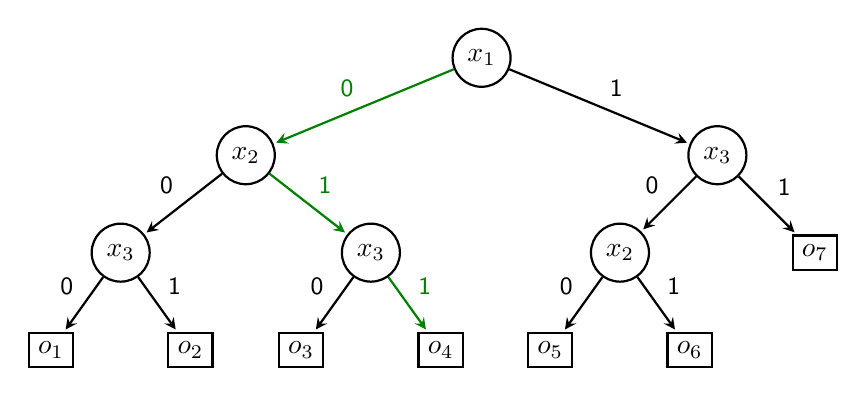
\begin{tikzpicture}[->,>=stealth,shorten >=1pt,auto,node distance=1.75cm, thick,main node/.style={scale=0.9,circle,draw,font=\sffamily\normalsize}]

        \node[circle, draw] (1)[] {$x_1$};

        \node[circle, draw] (2) [below left of=1, xshift=-50, ]{$x_2$};
        \node[circle, draw] (3) [below right of=1, xshift=50, ]{$x_3$};

        \node[circle, draw] (4) [below left of=2, xshift=-10, ]{$x_3$};
        \node[circle, draw] (5) [below right of=2, xshift=10, ]{$x_3$};
        \node[circle, draw] (6) [below left of=3, ]{$x_2$};
        \node[rectangle, draw] (7) [below right of=3]{$o_7$};

        \node[rectangle, draw] (8) [below left of=4, xshift=10]{$o_1$};
        \node[rectangle, draw] (9) [below right of=4, xshift=-10]{$o_2$};
        \node[rectangle, draw] (10) [below left of=5, xshift=10]{$o_3$};
        \node[rectangle, draw] (11) [below right of=5, xshift=-10]{$o_4$};
        \node[rectangle, draw] (12) [below left of=6, xshift=10]{$o_5$};
        \node[rectangle, draw] (13) [below right of=6, xshift=-10]{$o_6$};

        \path[every node/.style={font=\sffamily\small}]
            (1) edge[swap, color=Green]  node{0} (2)
            (1) edge node{1}(3)

            (2) edge[swap]  node{0} (4)
            (2) edge[color=Green]  node{1}(5)

            (3) edge[swap]  node{0} (6)
            (3) edge  node{1}(7)
            
            (4) edge[swap]  node{0} (8)
            (4) edge  node{1}(9)

            (5) edge[swap]  node{0} (10)
            (5) edge[color=Green]  node{1}(11)

            (6) edge[swap]  node{0} (12)
            (6) edge  node{1}(13)
        ;
    \end{tikzpicture}

    \caption{An example of decision tree of size 13 and depth 3. The green path shows the computation made for the input $x = 011$.}
\end{figure}

Decision trees give an easier way to describe the computation of an oracle Turing machine: if $M^B$ solves (or verifies) a problem $A$ then the $i$-th query made by the procedure corresponds to a variable $x_i$ for the decision tree where $x_i = 1$ if the query returns a positive result and 0 otherwise. In other words, the computation tree of an oracle Turing machine is actually a decision tree.

\begin{proposition}
    Given a search problem $A \in \mathsf{TFNP}$, there is an oracle Turing machine $M^B$ that solves (or verifies) $A$ if and only if there is a decision tree that solves (or verifies) $A$.
\end{proposition}

The above proposition gives a strong result that allows us to characterize black-box \TFNP through decision trees instead of oracles: \textit{any decision tree separation implies a relativized separation} \cite{proofs_circuits_communication, tfnp_characterization}. As in the communication complexity formulation, given a \TFNP problem $R$, we denote with $R^{dt}$ the equivalent $\TFNP^{dt}$ problem, where \textit{dt} stands for \textit{decision tree}. We will omit this notation when the context makes it clear.

\begin{definition}
    We define $\mathsf{FP}^{dt}$ as the set of query search problems $R = (R_n)_{n \in \N}$ for which there exists a polylogarithmic depth decision tree $T_n$ such that $T_n(x) = y$ if and only if $(x,y) \in R_n$. Likewise, we define $\mathsf{FNP}^{dt}$ as the set of query search problems $R = (R_n)_{n \in \N}$ for which there exists a polylogarithmic depth decision tree $T_y$ such that $T_y(x) = 1$ if and only if $(x,y) \in R_n$.
\end{definition}

Like protocols, in query search problems the certificate is the verifying decision tree itself. Decision tree reductions are based on a more fine-grained definition, where the function that maps inputs of the first problem to inputs of the second problem is computed by many decision trees with output $\{0,1\}$.

\begin{definition}
    A query search problem $R = (R_m)_{m \in \N}$, where $R_m \subseteq \{0,1\}^m \times O_m$ is said to be many-to-one reducible to a query search problem $S = (S_n)_{n \in \N}$, where $S_n \subseteq \{0,1\}^n \times O_n'$, if for all $m \in \N$ there is an $n \in \N$ for which there is a family of decision trees $T_i : \{0,1\}^m \to \{0,1\}$ for each $i \in [n]$ and a decision tree $T_y^o : \{0,1\}^m \to O_m$ for each $y \in O_n'$ such that:
    \[\forall x \in \{0,1\}^m \;\; (T(x), y) \in S \implies (x, T_y^o(x)) \in R\]
    where $T(x) := (T_1(x), \ldots, T_n(x))$.
\end{definition}

The difference in notation between $T_1, \ldots, T_n$ and $T_y^o$ underlines the fact that the former return a $\{0,1\}$ output, while the latter return an output in $O_n$. The \textit{size} of the reduction is the number of input bits to $S$, that being $n$. The \textit{depth} $d$ of the reduction is the maximum depth of any tree involved in the reduction, including each $T_i$ and each $T_y^o$. The complexity of the reduction is denoted as $S^{dt}_\leq(R)$ and it's equal $\log n + d$. A decision tree reduction is considered efficient if its complexity is polylogarithmic, i.e. equal to $O(\log^k n)$. 

\begin{definition}
    Given $S \in \mathsf{TFNP}^{dt}$, we define the class $S^{dt}$ as the subset of \textsf{TFNP}$^{dt}$ problems efficiently reducible through decision trees to the problem $S$, formally $S^{dt} = \{R \in \mathsf{TFNP} \mid S^{dt}_\leq(R) = O(\log^k n)\}$
\end{definition}

\section{Connections to Proof Complexity}

Like the white-box model, black-box total search problems can be studied under multiple lenses, such as \textbf{proof complexity}. This branch of complexity theory studies the complexity measures needed for a propositional formula to be proved by propositional proof systems, that being any system of rules that can prove the truthfulness of a propositional formula, i.e. a string made of logical operators applied on a set of $n$ variables, such as $F = x_1 \land (x_1 \to \lnot x_2 \lor x_3)$. Any statement can be encoded by propositional formulas, which is either a \textit{tautology} (a statement that is always true), a \textit{satisfiable} formula (a statement that can be true or false based on the assignment) or an \textit{unsatisfiable} formula (a statement that is always false). Proving that a formula $F$ is a tautology is equivalent to proving that $\lnot F$ is unsatisfiable.

Proof systems can be viewed as an algorithm that manipulates propositional formulas in order to produce a new one. When a formula $G$ is derived by the formula $F$ in the proof system $S$, we write $F \stackrel{S}{\vdash} G$. Proof systems must be \textit{sound}: if $F \stackrel{S}{\vdash} G$ then $G$ is a \textit{logical consequence} of $F$, which means that $F \to G$ is a tautology. In 1979, Cook and Reckhow gave the following formal definition of propositional proof system - often called Cook-Reckhow proof systems.

\begin{definition}
    A propositional proof system (or pps) is a polynomial time computabile surjective function $f : \Sigma^* \to \mathrm{TAUT}$, where $\mathrm{TAUT}$ is the set of logical tautologies.
\end{definition}

Given a formula $F \in \mathrm{TAUT}$ a string $s \in \Sigma^*$ and a proof system $f$, we say that $s$ encodes $F$ for the pps $f$ if it holds that $f(s) = F$. This idea justifies why we want proof systems to be surjective: any true statement must have a valid encoding in the proof system. This property is called \textit{completeness} of the proof system.

The most studied proof system is \textit{resolution} (or \textsf{Res}). Given a formula $F \in \mathrm{TAUT}$, this proof system is able to prove that it is indeed a tautology by proving that $\lnot F \in \mathrm{UNSAT}$. A \textit{CNF formula} $F$ is a conjunction of $m$ \textit{clauses} $C_1, \ldots, C_m$, where $C_i$ is a disjunction of $k_i$ \textit{literals}, that being either a variable defined on $F$ or its negation. For example, the following formula is in conjunctive normal form:
\[F = (x_1 \lor x_2 \lor \overline{x_3} \lor x_4) \land (x_1 \lor \vnot{x_2}) \land x_3\]

Any formula can be expressed as an equivalent CNF formula, making resolution a \textit{complete} and \textit{sound} proof system. Resolution proof are based on repeated applications of the following simple rule called the \textit{resolution rule}:
\[\dfrac{C \lor x \qquad D \lor \vnot x}{C \lor D}\]

Given a CNF formula $F = C_1 \land \ldots \land C_m$ and a clause $C$, we have that $F \stackrel{\mathsf{Res}}{\vdash} C$ if there is a sequence of clauses $D_1, \ldots, D_k$ such that $D_k = C$ and each $D_i$ in the sequence is either an \textit{axiom} of $F$ (meaning that $D_i = C_j$ for some $j$) or is obtained by applying the resolution rule on $D_p$ and $D_q$ for some $p,q < i$. Resolution is able to prove that a CNF formula $\lnot F$ is unsatisfiable by deriving the empty clause $\bot$ starting from the axioms of the formula itself. A Resolution proof is often referred to as a \textit{refutation}.

\begin{proposition}
    Given a CNF formula $F$, it holds that $F \in \mathrm{UNSAT}$ if and only if $F$ is refuted by Resolution
\end{proposition}

For example, given the following unsatisfiable CNF formula $(y \lor z) \land (y \lor \vnot{z}) \land (x \lor \vnot{y} \lor z) \land (\vnot{x} \lor z) \land \vnot{z}$, a Resolution proof is given by:
\[\begin{array}{lcl}
    D_1 & \vnot{z} & \text{Axiom} \\
    D_2 & (y \lor z) & \text{Axiom} \\
    D_3 & y & \text{Res. on $D_1, D_2$} \\
    D_4 & (x \lor \vnot{y} \lor z)  & \text{Axiom} \\
    D_5 & (x \lor \vnot{y}) & \text{Res. on $D_1, D_4$} \\
    D_6 & (\vnot{x} \lor z) & \text{Axiom} \\
    D_7 & \vnot{x} & \text{Res. on $D_1, D_6$} \\
    D_8 & \vnot{y} & \text{Res. on $D_5, D_7$} \\
    D_9 & \bot & \text{Res. on $D_3, D_8$} \\
\end{array}\]

which can also be graphically expressed as:

\begin{figure}[H]
    \centering
    
    \begin{tikzpicture}[-,>=stealth,shorten >=1pt,auto,node distance=2.25cm, thick,main node/.style={scale=0.9,circle,draw,font=\sffamily\normalsize}]
        \node (1) []{$\bot$};
        
        \node (2) at ($(1)+(-2,1.75)$){};
        \node (3) at ($(1)+(2,1.75)$){$\vnot{y}$};
    
        \node (4) [above left of=2]{};
        \node (5) [above right of=2]{};
    
        \node (6) [above of=3]{$\vnot{y} \lor x$};
        \node (7) [right of=6]{$\vnot{x}$};
        
        \node (8) [above left of=6]{$x \lor \vnot{y} \lor z$};
        \node (9) [above right of=6]{$\vnot{x} \lor z$};
    
        \node (11) [right of=9]{$\vnot{z}$};
        \node (12) [above left of=2]{$y$};
    
        \node (14) at ($(8)+(-2.4,0)$){$y \lor \vnot{z}$};
        \node (15) [left of=14]{$y \lor z$};
    
        \path[every node/.style={font=\sffamily\small}]
            (15) edge (12)
            
            (6) edge (3)
            (7) edge (3)
            
            (8) edge (6)
            (11) edge (6)
            
            (9) edge (7)
            (11) edge (7)
    
            (11) edge (12)
    
            (12) edge (1)
            (3) edge (1)
        ;
    \end{tikzpicture}
    
    \caption{Dag-like refutation of the previous formula}
\end{figure}

Through this representation, each refutation produces a directed acyclic graph (DAG), also knows as dag-like refutations. When each clause appears only once in a refutation, the latter is referred to as a tree-like refutation due to how the underlying graph is actually a tree.

\begin{figure}[H]
    \centering
    
    \begin{tikzpicture}[-,>=stealth,shorten >=1pt,auto,node distance=2.25cm, thick,main node/.style={scale=0.9,circle,draw,font=\sffamily\normalsize}]
    
        \node (1) []{$\bot$};
        
        \node (2) at ($(1)+(-2,1.75)$){$y$};
        \node (3) at ($(1)+(2,1.75)$){$\vnot{y}$};
    
        \node (4) [above left of=2]{};
        \node (5) [above right of=2]{};
    
        \node (6) [above of=3]{$\vnot{y} \lor z$};
        
        \node (8) [above left of=6]{$x \lor \vnot{y} \lor z$};
        \node (9) [above right of=6]{$\vnot{x} \lor z$};
    
        \node (11) [right of=9]{$\vnot{z}$};
    
        \node (14) at ($(8)+(-2.4,0)$){$y \lor \vnot{z}$};
        \node (15) [left of=14]{$y \lor z$};
    
        \path[every node/.style={font=\sffamily\small}]
            (14) edge (2)
            (15) edge (2)
    
            (8) edge (6)
            (9) edge (6)
    
            (6) edge (3)
            (11) edge (3)
    
            (2) edge (1)
            (3) edge (1)
        ;
    \end{tikzpicture}
    
    \caption{Tree-like refutation of the previous formula}
\end{figure}

This subset of proofs defines a more specific proof system called \textit{Tree-like Resolution} (or \textsf{TreeRes}). Generally, this type of refutations require trees of exponential size and polynomial depth compared to the number of variables defined on the formula itself. A standard result in proof complexity states that Resolution and Tree-like resolution are separated, meaning that some proofs are easy for the former and hard for the latter, making Resolution a stronger proof system.

But why are we interested in proving or refusing propositional formulas? We discussed how the $\mathrm{SAT}$ problem is \textsf{NP}-Complete. This clearly implies that the problem $\overline{SAT}$ is \textsf{coNP}-Complete. This fact can be used to show that $\overline{SAT} \leq_m \mathrm{UNSAT} \leq_m \mathrm{TAUT}$, implying that both $\mathrm{UNSAT}$ and $\mathrm{TAUT}$ are also \textsf{coNP}-Complete. If we can show that either one of these problems is also in $\mathsf{NP}$ then we would have an answer to the $\mathsf{NP} \stackrel{?}{=} \mathsf{coNP}$ question.

Proof systems are essential to work on this question: given the encoding $s$ of a tautology $F$, a verifier can follow the rules defined by a proof system in order to prove that $F$ is indeed a tautology. In this case, $s$ serves as a certificate for $F$ while the pps defines the algorithm. We give the following equivalent definition of propositional proof system equivalent to the previous one.

\begin{definition}
    A propositional proof system (or pps) is a polynomial verifier $V$ such that $F \in \mathrm{TAUT}$ if and only if there is a string $s \in \Sigma^*$ such that $V(F,s) = 1$.
\end{definition}

On first glance, one could think that this definition imply that any complete and sound pps proves that $\mathrm{TAUT} \in \mathsf{NP}$. However, we must also consider the size of such certificates: in order to be an efficient verifier, the size of the certificates must be polynomially bounded by the size of $F$. In other words, it must hold that $\abs{s} = O(\abs{F}^k)$ for some $k \in \N$. This means that in order to prove that $\mathsf{NP} \neq \mathsf{coNP}$ (which is equivalent to proving that $\mathrm{TAUT} \in \mathsf{NP}$) we must find a \textit{polynomially bounded proof system}, a pps that uses only polynomially bounded certificates for all tautologies.

\begin{proposition}
    There is a polynomially bounded proof system if and only if $\mathsf{NP} \neq \mathsf{coNP}$.
\end{proposition}

We already discussed how researches believe that $\mathsf{NP} \neq \mathsf{coNP}$ is the expected answer to the conjecture. In order to prove this, we would have to prove that there cannot be a polynomially bounded pps. Proving this statement is no easy task: we would have to prove that there is a particular formula $F$ that strictly requires an exponential size encoding for every discovered and undiscovered proof system. Even thought this result seems out of reach, proof complexity is highly related to other branches of complexity theory, including our case!

In order to get to this relation between proof complexity and $\mathsf{TFNP}^{dt}$, we will restrict our focus to \textbf{conjunctive normal form (CNF) formulas}. 

By construction, a CNF formula can be unsatisfiable if and only if for all assignments $\alpha(x_1, \ldots, x_n)$ there is a clause $C_i$ that is false. It's easy to see this fact implies that any CNF formula gives rise to an associated search problem: finding a falsified clause inside the formula (if there is any) for each possible assignment.

\begin{definition}
    Given a CNF $F = C_1 \land \ldots \land C_m$ over $n$ variables, we define $\mathrm{Search}(F)$ as the following search problem: given an input assignment $\alpha(x_1, \ldots, x_n)$, return an index $i$ such that the assignment falsifies $C_i$.
\end{definition}

This problem is usually referred to as the \textit{false clause search problem}. 
When $F$ is an unsatisfiable CNF formula, $\mathrm{Search}(F)$ is clearly a total search problem since for any input assignment there will always be an unsatisfied clause. Moreover, the search problem of any unsatisfiable formula can easily be solved (or verified) by a decision tree for any formula $F$: if the assignment $\alpha(x_1 = b_1, \ldots, x_n = b_2)$ falsifies the clause $C_i$, define a path $x_1 = b_1, \ldots, x_n = b_n$ on the decision tree and let $C_i$ be the output of such path. In other words, for all $\lnot F \in \mathrm{TAUT}$ it holds that $\mathrm{Search}(F) \in \mathsf{TFNP}^{dt}$. 

\begin{figure}[H]
    \centering
    
    \begin{tikzpicture}[-,>=stealth,shorten >=1pt,auto,node distance=2.25cm, thick,main node/.style={scale=0.9,circle,draw,font=\sffamily\normalsize}]
    
        \node (1)[circle, draw]{$y$};
        
        \node (2) at ($(1)+(-2,-1.75)$) [circle, draw]{$z$};
        \node (3) at ($(1)+(2,-1.75)$) [circle, draw]{$z$};
    
        \node (4) [below left of=2]{};
        \node (5) [below right of=2]{};
    
        \node (6) [below of=3, circle, draw]{$x$};
        
        \node (8) [below left of=6, rectangle, draw]{$x \lor \vnot{y} \lor z$};
        \node (9) [below right of=6, rectangle, draw]{$z \lor \vnot{x}$};
    
        \node (11) [right of=9, rectangle, draw]{$\vnot{z}$};
    
        \node (14) at ($(8)+(-2.4,0)$) [rectangle, draw]{$y \lor \vnot{z}$};
        \node (15) [left of=14, rectangle, draw]{$y \lor z$};
    
        \path[every node/.style={font=\sffamily\small}]
            (14) edge [swap] node{1} (2)
            (15) edge node{0} (2)
    
            (8) edge node{0}(6)
            (9) edge node[swap]{1}(6)
    
            (6) edge node{0}(3)
            (11) edge [swap] node{1}(3)
    
            (2) edge node {0} (1)
            (3) edge node [swap] {1} (1)
        ;
    \end{tikzpicture}
    
    \caption{Decision tree for the unsatisfiable formula $(y \lor z) \land (y \lor \vnot{z}) \land (x \lor \vnot{y} \lor z) \land (\vnot{x} \lor z) \land \vnot{z}$}
    \end{figure}

    In a similar fashion, we can show that any total query search problem $R$ can be associated with the search problem of the formula $F$ that describes the set of decision trees that verify $R$.

Consider a decision tree $T$ made of the paths $p_1, \ldots, p_k$, each leading to the leaves $\ell_1, \ldots, \ell_k$. The DNF encoding of $T$, denoted with $D_T$, is the disjunction over the conjunction of the literals $\alpha_1, \ldots, \alpha_h$ along each of the accepting paths in $T$. In other words, we have that $D_T = p_1 \lor \ldots \lor p_k$ where each $p_i = \alpha_1 \land \ldots \land \alpha_h \land \ell_i$ is an accepting path of $T$. By De Morgan's theorem, $\vnot{D_T}$ is a CNF.

\begin{proposition}
    \label{Rdt = Search(F)}
    Given a total query search problem $R \subseteq \{0,1\}^n \times O$, for each $n \in \N$ there exists an unsatisfiable CNF formula $F_n$ defined over $\abs{O}$-many variables such that $R_n = \mathrm{Search}(F_n)$. This formula is called canonical CNF encoding of $R_n$.
\end{proposition}

\begin{proof}
    Since $R = (R_n)_{n \in \N} \in \TFNP^{dt}$, for each $y \in O_n$ there is a $\mathrm{polylog}(n)$-depth decision tree $T_y$ that verifies $R_n$. Consider the CNF $F_n := \bigwedge\limits_{y \in O_n} \vnot{D_{T_y}}$. Since $R$ is a total search problem, for each input $x$ there is a valid output, implying that at least one tree $T_y$ will have an accepting path, meaning that $D_{T_y}(x) = 1$ and therefore $\vnot{D_{T_y}}(x) = 0$, concluding that $F_n$ is unsatisfiable. Moreover, this formulation also concludes that:
    \[(x,y) \in R_n \iff T_y(x) = 1 \iff \vnot{D_{T_y}}(x) = 0 \iff (x,y) \in \mathrm{Search}(F_n)\]
    and thus that $R_n = \mathrm{Search}(F_n)$.

\end{proof}

This result clearly implies that $(R)_{n \in \N} = (\mathrm{Search}(F_n))_{n \in \N}$, where $F_1, F_2, \ldots$ is a family of CNF formulas, and by extension that black-box \TFNP is exactly \textit{the study of the false clause search problem}. Like in the white-box case, the upshot is that it is sufficient to restrict our interests on the study of search problems associated to unsatisfiable CNF formulas.

Through this connection, Göös et al. \cite{adventures_monotone_tfnp} showed that many important proof systems are characterized by an associated $\mathsf{TFNP}^{dt}$ search problem and vice versa. Given a proof system $P$ and an unsatisfiable CNF formula $F$, the \textbf{complexity} required by $P$ to prove $F$ is given by:
\[P(F) := \min\{\log \mathrm{size}(\Pi) + \mathrm{deg}(\Pi) : \Pi \text{ is a $P$-proof of } F\}\]
where $\mathrm{size}(\Pi)$ is the sum of the sizes of all the formulas inside it, or in other words the total number of symbols in $\Pi$, and $\mathrm{deg}(\Pi)$ is the \textit{degree} of $\Pi$ associated to $P$, which varies from proof system to proof system. This degree measure will be specified for the proof systems analyzed in following sections.

To make things more readable, we will refer to $\mathrm{Search}(F)$ as $S_F$. Since each $\TFNPdt$ problem is equivalent to $S_F$ for some formula $F$, the complexity parameter defined above can be used to give another characterization of $\TFNPdt$ problems.

\begin{definition}
    We say that a proof system $P$ \textbf{characterizes} a $\TFNPdt$ problem $R$ (and reflexively that $R$ characterizes $P$) if it holds that \[R^{dt} = \{S_F : P(F) = \mathrm{polylog}(n)\}\]
    where $F = F_1, F_2, \ldots$ is a family of formulas. In a stronger sense, it holds that $R^{dt}(S_F) = \Theta(P(F))$. 
\end{definition}

Most of the \TFNP subclasses discussed in previous sections has been shown to have a characterizing proof system:
\begin{itemize}
    \item $\mathrm{FP}^{dt}(S_F) = \Theta(\mathrm{TreeRes}(F))$ \cite{search_problems_dt_model}
    \item $\mathrm{PLS}^{dt}(S_F) = \Theta(\mathrm{Res}(F))$  \cite{approx_counting}
    \item $\mathrm{PPA}^{dt}(S_F) = \Theta(\F_2\mathrm{\text{-}NS}(F))$ \cite{adventures_monotone_tfnp}
    \item $\mathrm{PPADS}^{dt}(S_F) = \Theta(\mathrm{unary\text{-}NS}(F))$ \cite{separations_proof_complexity}
    \item $\mathrm{PPAD}^{dt}(S_F) = \Theta(\mathrm{unary\text{-}SA}(F))$ \cite{separations_proof_complexity}
    \item $\mathrm{SOPL}^{dt}(S_F) = \Theta(\mathrm{RevRes}(F))$ \cite{separations_proof_complexity}
    \item $\mathrm{CLS}^{dt}(S_F) = \Theta(\mathrm{RevResT}(F))$ \cite{separations_proof_complexity}
\end{itemize}

\newpage

\section{Canonical Proof Systems}

In an intuitive way, this characterization also shows that \textit{any} $\TFNPdt$ problem can be transformed into a proof system for refuting unsatisfiable CNF formulas of polylogarithmic width: since any $\TFNPdt$ is equivalent to the search problem for some unsatisfiable CNF formula, any efficient decision tree reduction between problems is nothing more than an efficient proof in the characterizing proof system and vice versa. To formalize this idea, we introduce the concept of \textbf{reductions between CNF formulas} \cite{tfnp_characterization}.

Suppose that $C$ is a clause over $n$ variables and that $T = (T_i)_{i \in [n]}$ is a sequence of depth-$d$ decision trees, where $T_i : \{0,1\}^{n'} \to \{0,1\}$. We refer to $C(T)$ as the CNF formula obtained by substituting each variable $x_i$ in $C$ with the associated tree $T_i$ and rewriting the result as a CNF, or more conveniently:
\[C(T) := \bigwedge_{i \in [n]} \, \bigwedge_{\substack{r \,:\, \text{rejecting} \\ \text{path of $T_i$}}} \overline{r}\]

\begin{definition}
    Let $F = C_1 \land \ldots \land C_{m_F}$ be an unsatisfiable CNF over $n_F$ variables. We say that a CNF formula $H$ made of $m_H$ clauses over $n_H$ variables reduces to $F$ via depth-$d$ decision trees if there exist two sequences of depth-$d$ decision trees $T = (T_i)_{i \in [n_F]}$ and $T' = (T_j^o)_{j \in [m_F]}$, where $T_i : \{0,1\}^{n_H} \to \{0,1\}$ and $T_j^o : \{0,1\}^{n_H} \to [m_H]$, such that given the following formula:
    \[F_H := \bigwedge_{j \in [m_F]} \,\bigwedge_{\substack{p \,:\; \text{path} \\ \text{in } T_j^o}} C_i(T) \lor \overline{p}\]
    it holds that if $F$ is unsatisfiable then $F_H$ is unsatisfiable and by consequence that $H$ is unsatisfiable. 
\end{definition}

In particular, we notice that $F_H$ can also be written as a CNF by simply distributing each $\overline{p}$ inside $C_i(T)$. Each clause $C_i(T) \lor \overline{p}$ must be either tautological (since it could contain a variable and its negation) or a weakening of the corresponding clause of $H$ indexed by the label at the end of the path $p$. Moreover, we notice that through this formulation any depth-$d$ decision tree reduction from $\mathrm{Search}(H)$ to $\mathrm{Search}(F)$ induces the search problem $\mathrm{Search}(F_H)$.

Reductions between CNF formulas imply that reductions between search problems reduction are actually a proof system. In particular, given a problem $\mathrm{Search}(F) \in \TFNPdt$, the \textbf{canonical proof system} of such problem, denoted with $P_F$ proves an unsatisfiable formula $H$ over $n_H$ variables if $H$ is reducible to an instance of $F$ over $n_F$ variables. A $P_F$-proof of $H$ consists of the decision trees that make such reduction possible. The \textit{size} of such proof is given by $n_F$, while the \textit{degree}, or \textit{depth} in this case, is given by the maximum depth among the involved decision trees. Hence, the $P_F$ complexity of $H$ is given by:
\[P_F(H) := \min\{\log n_H + \mathrm{depth}(\Pi) : \Pi \text{ is a $P_F$-proof of } H\}\]

These proof systems are \textit{sound}, since by construction any valid substitution of an unsatisfiable CNF formula is also unsatisfiable, and also \textit{efficiently verifiable}, since it suffices to check that each of the clauses of $F_H$ is either tautological or a weakening of a clause in $H$, which can be done polynomially in size of the proof.

From this definition of canonical proof system, the following theorem is given for free. This theorem plays a crucial role in $\TFNPdt$ characterization through proof complexity, stating that $P_F$ has a short proof of $H$ if and only if $\mathrm{Search}(H)$ efficiently reduces to $\mathrm{Search}(F)$. 

In particular, we observe that \textbf{any characterizing proof system} is actually the canonical proof system of the associated search problem, a result that follows from the two definitions. In other words, proving a formula in a characterizing proof system automatically gives a reduction to the corresponding complete search problem.

\begin{theorem}
    Let $\mathrm{Search}(F) \in \TFNPdt$ and let $H$ be an unsatisfiable CNF formula. The two following results hold:
    \begin{enumerate}
        \item If $H$ has a size $s$ and depth $d$ proof in $P_F$ then $\mathrm{Search}(H)$ has a size $O(s)$ and depth $d$ reduction to $S_F$
        \item If $\mathrm{Search}(H)$ has a size $s$ and depth $d$ decision tree reduction to $\mathrm{Search}(F)$ then $H$ has a size $s2^{O(d)}$ and depth $d$ proof in $P_F$
    \end{enumerate}
    In particular, this implies that $\mathrm{Search}(F)^{dt}(\mathrm{Search}(H)) = \Theta(P_F(H))$.
\end{theorem}

\begin{proof}
    Suppose that $T = (T_i)_{i \in [n_F]}$ and $T' = (T_j^o)_{j \in [m_F]}$ is a $P_F$ proof of $H$ of size $s$ and depth $d$. Given any assignment $x$ such that $(x, i) \in \mathrm{Search}(F)$, let $C_i$ be the clause of $F$ falsified by $T_1(x), \ldots, T_{n_F}(x)$ and let $p$ be the path followed by $T_i^o(x)$. It's easy to see that a clause of the formula $C_i(T) \lor \overline{p}$ must be falsified by $x$. In particular, such clause is also the weakening of the $T_i^o(x)$-th clause of $H$, concluding that $(x, T_i^o(x)) \in \mathrm{Search}(H)$. In other words, the $P_F$ proof of $H$ corresponds to a reduction from $\mathrm{Search}(H)$ to $\mathrm{Search}(F)$ of size $n_F = O(s)$ and depth $d$.

    Vice versa, suppose that $T = (T_i)_{i \in [n_F]}$ and $T' = (T_j^o)_{j \in [m_F]}$ is a decision tree reduction from $\mathrm{Search}(H)$ to $\mathrm{Search}(F)$ of size $s$ and depth $d$. Then, we can construct $F_H$ as previously described through the use of these decision trees. Let $L$ be a clause of $C_i(T)$ for some $i \in [m_F]$ and let $p$ be any path in $T_i^o$. If the formula $C_i(T) \lor \overline{p}$ is tautological, then it can be ignored since $F_H$ is a CNF. Otherwise, let $x$ be an assignment that falsifies $L \lor \overline{p}$. Then, it holds that $T_1(x), \ldots, T_{n_F}(x)$ falsifies $C_i(T)$ and that $T_i^o(x)$ follows path $p$. Thus, the $T_i(x)$-th clause of $\overline{H}$ must also be false, implying that $L \lor \overline{p}$ is a weakening of such clause. This concludes that $F_H$ is a $P_F$-proof of $H$ of depth at most $d$ (due to how $F_H$ is constructed) and thus that the size is at most $s2^{O(d)}$.

\end{proof}

\cleardoublepage